\documentclass{standalone}
\usepackage{tikz}
\usetikzlibrary{decorations.pathreplacing}
\begin{document}

            % TIKZ
            %$\left\{
                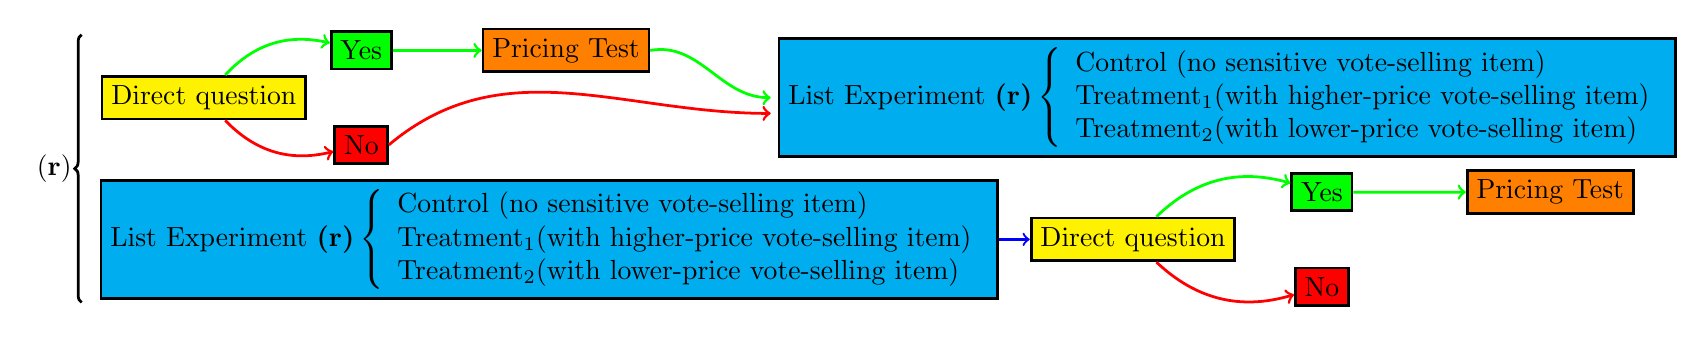
\begin{tikzpicture}[
                %scale=2
                scale=.2,
                line width=1pt] %

% random
\draw[decoration={brace,mirror,raise=10pt},decorate]
  (-28,-2) -- node[black,midway,xshift=-0.7cm] {({\bf r})} (-28,-19);

                    % 1
                    \node[draw,align=center,fill=yellow,text=black] (DQ1) at (-22,-6) {Direct question}; % 1
                    
                    \node[draw,align=center,fill=green,text=black] (YES1) at (-12,-3) {Yes}; % 1
                    \node[draw,align=center,fill=red,text=black] (NO1) at (-12,-9) {No}; % 1


                    \node[draw,align=center,fill=orange,text=black] (PE1) at (1,-3) {Pricing Test}; % 1

                    \node[draw,align=center,fill=cyan,text=black] (LE1) at (43,-6)   {List Experiment  % 1
                    $
                  \mbox{{\bf (r)}}
                  \left\{
                        \begin{array}{llc}
                            \mbox{Control (no sensitive vote-selling item)}\\
                            \mbox{Treatment}_{1} \mbox{(with higher-price vote-selling item)}\\
                            \mbox{Treatment}_{2} \mbox{(with lower-price vote-selling item)}\\
                          \end{array}
                    \right.
                    $};

                    %\draw[->,draw=blue,thick] (DQ1) to (PE1);
                    %\draw[->,draw=blue,thick] (PE1) to (LE1);
                    \path [green,bend left,->] (DQ1) edge (YES1);
                    \path [green,->] (YES1) edge (PE1);
                    \path [green, out=10,in=180, ->] (6.35,-3) edge (14,-6);


                    \path [red,bend right,->] (DQ1) edge (NO1);
                    \path [red, out=40,in=180, ->] (-10.25,-9) edge (14,-7);






                    % 2
                    \node[draw,align=center,fill=cyan,text=black] (LE2) at (-.05,-15) {List Experiment  % 1
                    $
                    \mbox{{\bf (r)}}
                    \left\{
                        \begin{array}{llc}
                            \mbox{Control (no sensitive vote-selling item)}\\
                            \mbox{Treatment}_{1} \mbox{(with higher-price vote-selling item)}\\
                            \mbox{Treatment}_{2} \mbox{(with lower-price vote-selling item)}\\
                          \end{array}
                    \right.
                    $};
                   

                    \node[draw,align=center,fill=yellow,text=black] (DQ2) at (37,-15) {Direct question}; % 2
                    \node[draw,align=center,fill=green,text=black] (YES2) at (49,-12) {Yes}; % 2
                    \node[draw,align=center,fill=red,text=black] (NO2) at (49,-18) {No}; % 2
                    \node[draw,align=center,fill=orange,text=black] (PE2) at (63.5,-12) {Pricing Test}; % 2



                    \draw[->,draw=blue,thick] (LE2) to (DQ2); % OK

%
                    \path [green,bend left,->] (DQ2) edge (YES2);
                    \path [green,->] (YES2) edge (PE2);


                    \path [red,bend right,->] (DQ2) edge (NO2);
                    %\path [red, out=40,in=180, ->] (-10.25,-9) edge (14,-7);

                    \end{tikzpicture}
               % \right.$

\end{document}